\section{Literature review}

As discussed before, this project aims to develop a system for optical Braille character detection, translation to English text, correction of the text, and finally conversion of the text to speech. This literature review examines existing research and technologies in Optical Braille Character Recognition (OBR), Braille recognition and translation, text correction algorithms, and text-to-speech (TTS) systems, highlighting their relevance and application to this project.\\


\subsection{Optical Braille Character Recognition (OBR)}

Numerous studies have addressed the problem of optical Braille detection, leading to the development of various methods for detecting and translating Braille into text. Over the years, continuous research has significantly improved accuracy, approaching near perfection. This progress has been achieved through techniques such as object detection using support vector machines, various image processing steps and filters, and machine learning, particularly with the recent advancements in artificial intelligence (AI) and deep learning.
\\
In this section, we will discuss some of these methods. We will begin with the image preprocessing steps and the filters employed in previous research.

\textbf{
\subsubsection{Image Acquisition}
}
Different mechanisms for image acquisition have been proposed in various studies. For instance, the paper titled "Image Processing Techniques for Braille Writing Recognition" by Néstor Falcón et al. [1] highlights the use of a flat-bed scanner instead of a digital camera. The choice of a flat-bed scanner is justified by its cost-effectiveness, versatility for other applications, and ease of use. The system described in the paper is capable of working with images of different resolutions, specifically adjusting images through interpolation methods to resize input images to a standard resolution, typically around 100 dots per inch (dpi). 

In the study titled "Analysis of Scanned Braille Documents" by Ritchings et al. [12], the methodology for optical Braille detection involves scanning Braille documents at 100 dpi to produce gray-scale images with 16 levels. This configuration was selected through empirical testing to optimize results while minimizing data size. The gray-scale variations in the scanned images reflect the intensity of reflected light, influenced by protrusions and depressions on the document's surface. \\
\textbf{
\subsubsection{Preprocessing}
}
\paragraph{In their paper, Al-Salman et al. [3] outline essential preprocessing steps for optical Braille recognition:}
In preprocessing the image for optical Braille recognition, the initial step involves converting colored images, typically stored in 3-D arrays, into 2-D grayscale arrays. This simplification streamlines processing and boosts computational efficiency, ensuring that pixel values uniformly span from 0 to 255. Following this, the image frame is cropped to eliminate unwanted black or white borders that may interfere with subsequent processing steps. This is achieved by calculating the average gray level across the entire image, as well as individually for each row and column. Rows or columns exhibiting an average gray level deviating more than 15\% from the image's overall average are identified and cropped out. Finally, image thresholding categorizes each pixel in the grayscale array into bright, dark, or gray categories based on predefined thresholds. Pixels with values 32 and above are classified as bright, those with values 23 and below as dark, and those between 23 and 32 as gray, setting the stage for subsequent stages of Braille dot detection and symbol recognition.\\

\paragraph{Antonacopoulos and Bridson [2] propose a series of preprocessing steps tailored for robust Braille recognition:}
Initially, they advocate for reducing the image's greylevels to three categories—shadows, light areas, and background—to enhance clarity and facilitate subsequent analysis. Next, a local adaptive thresholding approach is implemented to accommodate varying light conditions across the image. This method divides the image into 32x32 pixel regions, with threshold values dynamically adjusted based on the observed greylevel ranges within each region. This ensures accurate segmentation of features such as whole dots, highlights, shadows, and background. As a result of these preprocessing steps, the image is transformed to distinctly display shadows as black regions, highlights as white regions, and the majority of mid-grey areas representing the background. These enhancements prepare the image effectively for further stages of Braille dot detection and symbol recognition.\\

\paragraph{In their comprehensive review, Isayed and Tahboub [4]}
 compare various optical Braille recognition algorithms based on several criteria. They analyze algorithms across different publishing years, evaluating advancements in technology over time. The study also considers the diversity in image acquisition techniques, examining the use of flatbed scanners versus digital cameras. Algorithms are categorized according to their ability to handle single-sided or double-sided Braille pages, highlighting the versatility and adaptability of each approach. Moreover, the review delves into image pre-processing techniques employed by these algorithms, such as grayscale conversion, frame cropping, and adaptive thresholding methods, which play crucial roles in enhancing the accuracy of Braille character recognition systems. This comparative analysis provides valuable insights into the evolution and effectiveness of optical Braille recognition technologies, offering guidance for future research and development in the field.


These preprocessing techniques are crucial for preparing scanned Braille documents for subsequent recognition and translation processes, ensuring accurate and efficient optical Braille recognition systems. 
\\
\subsubsection{Image Alignment and De-skewing}

After discussing image preprocessing techniques in optical Braille recognition, the next critical step involves addressing the challenge of de-skewing rotated images. De-skewing is essential because scanned documents often suffer from rotational variations, which can affect the accuracy of subsequent recognition processes. Various methods and algorithms have been developed to automatically detect and correct these rotations, ensuring that Braille characters are accurately interpreted regardless of their orientation on the scanned page. 

\paragraph{
Isayed and Tahboub [4] discuss various methods to tackle the skewing problem in optical Braille recognition:\\}

They highlight the \textbf{Linear Regression Method}, which seeks to find the optimal line that fits the Braille dots using the formula Y=BX+A.\\

Another approach involves calculating \textbf{Standard Deviation}. This method rotates the image by an angle $\theta$ and computes new values of  $\overline{X}$ and S for each row. The optimal angle $\theta$ is determined based on maximizing S.  The calculation of the standard equation can be done using the following equations:

\begin{equation}
s = \sqrt{\frac{1}{n} \sum_{i=1}^{n} (x - \bar{x})^2}
\end{equation}

\begin{equation}
\bar{x} = \frac{1}{n} \sum_{i=1}^{n} x_i
\end{equation}

where x is the coordinate on the horizontal axis\\
\\Another solution was mentioned and it is the solution we decided to go with in our project is the \textbf{Hough Transform Algorithm} introduced by Antonacopoulos and Bridson [2]. It offers a robust solution to the skewing problem. This technique detects lines in the image space and can be adapted to identify the optimal rotation angle. 


 \textbf{
\subsection{ Using Image Processing to detect Braille symbols}
}

After addressing image skewing challenges, symbol detection is the next critical step in optical Braille recognition. This phase involves extracting individual Braille dots or clusters from preprocessed images to facilitate accurate character recognition. Techniques such as pattern recognition algorithms, contour detection, and template matching are utilized to identify and isolate Braille features amidst background noise. It is essential to differentiate between single-sided and double-sided Braille images, as the presence of Braille dots on both sides impacts the detection and segmentation processes significantly. This section explores the methodologies and advancements in dot detection, emphasizing their role in preparing data for subsequent recognition and translation processes.
\\
\paragraph{ Falcón et al. [1]}
 leverage shadows cast by the skew angle of light beams in reflection scanners to differentiate between front and back side Braille dots. Their method involves manipulating "islands" of white pixels: shifting them downwards by 4 pixels to extract front side dots and upwards by 4 pixels to extract back side dots. This "shift and overlap" technique efficiently separates the document sides without the need for sequential image matrix reading, ensuring simplicity and speed in processing.

\clearpage
\begin{figure}
\centering
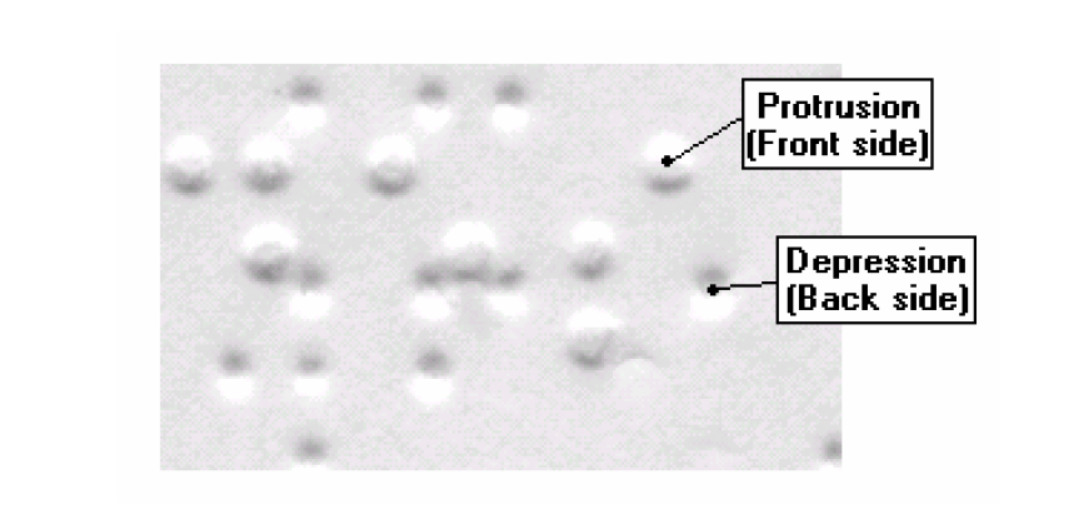
\includegraphics[width=1\linewidth]{front and backPNG.PNG}
\caption{front and back braille page}
\label{fig:acc}
\end{figure}

 Furthermore, the algorithm detects and corrects the document's skew angle using horizontal histogram analysis and calculation of mass centers. Notably, not all dots are detected using the overlapping process due to their small size or insufficient shadow overlap within the 4-pixel threshold. To address this, they introduce an adaptive algorithm to construct a Braille grid from the detected dots. 
 


In the grid construction phase, the adaptive algorithm starts by identifying columns aligned with the normalized distances between Braille dots. The initial stage focuses on grouping dots into vertical columns that conform to typical Braille dot spacing patterns. Subsequently, the algorithm adjusts the grid to accommodate variations in document layout, ensuring flexibility in column placement to handle slight deviations.
\begin{figure}[!ht]
\centering
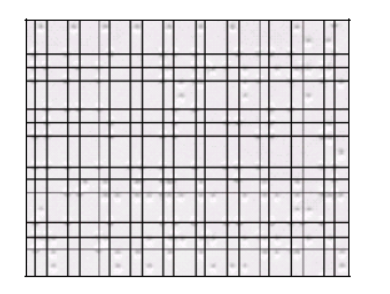
\includegraphics[]{grif.PNG}
\caption{the grid constructed for the detection}
\label{fig:acc}
\end{figure}


Similarly, the algorithm proceeds to establish rows aligned with Braille row patterns, completing the grid structure by integrating detected columns and rows. This flexible grid construction approach preserves the original document layout, enabling accurate representation of Braille positions without compromising format integrity.

Once the grid is established, the system employs dilation techniques to expand the search area around potential Braille dot positions. This step optimizes the system's efficiency by focusing detailed scrutiny on areas identified as potential Braille dot locations. Only positions that match the expected Braille dot criteria are validated, ensuring accurate detection while filtering out false detections that do not align with valid Braille dot locations.

Since the mentioned works essentially rely on snapping Braille points to the grid, they mostly work with images obtained with a scanner.

This methodical approach underscores the intelligence of the overall system, prioritizing time efficiency through targeted dot validation and ensuring robust detection of genuine Braille characters within scanned documents.

 
\paragraph{ W.D. Chamalee et al. [5] }
propose an algorithm designed to identify individual Braille characters on embossed printed paper using image processing techniques. Their method utilizes a stripping approach, which involves several key techniques such as dilation, standard distance ratios, and a vertical filling algorithm.

The algorithm is specifically tailored for embossed printed papers written in the Sinhalese language. It has been rigorously tested and demonstrates an impressive average accuracy of 99.2\%. This high accuracy underscores the effectiveness of their approach in reliably extracting Braille characters from printed documents, thereby enabling efficient and accurate optical Braille recognition.

\textbf{
\subsection{Using Convolutional Neural Networks (CNNs) for detecting Braille symbols}
}

\paragraph{In his paper on Optical Braille Recognition Using Object Detection CNN, Ilya G. Ovodov [6]}
 notes that while convolutional neural networks (CNNs) have significantly advanced image recognition in recent years, their application specifically to optical Braille recognition (OBR) is limited. He highlights sparse literature on the use of deep learning techniques, particularly fully connected neural networks (FCNs), in OBR. This observation underscores the nascent exploration of neural network applications in Braille recognition compared to their widespread adoption in general image recognition tasks.

Ovodov highlights the significant progress in computer vision, particularly in object detection, driven by Convolutional Neural Networks (CNNs) since their introduction by LeCun in 1989 and their explosion in popularity from 2012 onwards. Initially, CNN-based solutions for object detection involved separate processes for region proposal and object classification. Later advancements, such as Single Shot Multibox Detector (SSD) and You Only Look Once (YOLO), introduced the concept of one-stage detectors. These models generate a feature map where each point corresponds to a region of interest in the image. Anchors, predefined sizes for objects, are used to predict bounding box adjustments, object presence (confidence), and object class simultaneously. RetinaNet further improves upon these methods with the FocalLoss function, enhancing performance on challenging cases. Ovodov utilized these advanced CNN architectures for object detection in his research.

Ovodov's approach differs from traditional methods by directly detecting whole Braille symbols and recognizing them simultaneously using an object detection CNN. Each Braille character is assigned a class label ranging from 1 to 63 based on its composition of raised dots. The input images are scaled to 100 dpi, resulting in a resolution of 864x1150 pixels for standard A4 pages. Braille characters are identified with horizontal spacing of approximately 25 points and line spacing of about 40 points.

For implementation, Ovodov uses the RetinaNet CNN architecture with optimizations to handle the specific characteristics of optical Braille recognition. The architecture is simplified to reduce execution time, particularly focusing on non-maximum suppression (NMS) operations. A single "output to class + box subnet" is employed at the layer level with feature map cells of size 16x16 pixels, ensuring coverage of each Braille character. Only one anchor per grid cell, sized close to expected character dimensions, is utilized to further optimize performance.

To address potential overlap issues inherent in object detection, especially with small and uniformly sized objects like Braille characters, Ovodov lowers the Intersection over Union (IOU) threshold to 0.02 during NMS. This adjustment minimizes filtering errors and maintains high recognition quality despite detector imperfections.

These modifications significantly reduce computational time while preserving robust recognition capabilities tailored specifically for optical Braille recognition tasks.



\subsection{Recognition of Braille Symbols}

In optical Braille recognition, the recognition phase follows the detection of Braille symbols from scanned images. Unlike traditional approaches that separate stages for dot detection, grid restoration, and character combination, modern methods aim to directly recognize whole Braille symbols in a single step. This streamlined approach enhances efficiency and accuracy by leveraging advanced computational techniques tailored for Braille reading systems.

The recognition process involves assigning each detected Braille symbol a specific class label that corresponds to its Braille character representation. This classification allows for seamless translation into textual or auditory formats, ensuring accessibility for visually impaired individuals. The recognition algorithms analyze the spatial arrangement of dots within each symbol, interpreting their positions and configurations to determine the corresponding Braille character.

\paragraph{ Néstor Falcón et al. [1] }
describe a method where the final image, containing Braille dots represented as spots, undergoes thorough analysis for text segmentation into rows and characters. Utilizing the Braille grid previously constructed, which marks all positions of Braille dots, each character is then converted into a binary number based on the active dots present.

The segmentation process assigns a unique binary representation to each Braille character, leveraging a straightforward coding scheme that translates the presence of raised dots into '1's and absence into '0's. For example, the character 'r' in Braille, represented as '111010', illustrates this binary coding method where each '1' corresponds to an active dot ('mountain') on the Braille sheet.

This binary representation ensures language independence within the system, allowing for straightforward configuration adjustments to accommodate different alphabets or languages. Each character's binary number is then translated into its equivalent letter in standard text format, producing a final output in the form of a text file.

This approach not only simplifies the recognition and translation of Braille characters but also facilitates the seamless integration of optical Braille recognition systems into diverse linguistic environments.

\paragraph{In their paper "Deep Learning Strategy for Braille Character Recognition," Tasleem Kausar and colleagues [7]}
 propose a deep CNN model for Braille character recognition. The model comprises two main layers: feature extraction and classification. For feature extraction, they employ established deep CNN networks such as VGG16, ResNet50, InceptionV3, and DenseNet201, modifying the final layers with an IRB (Inverted Residual Block) module to enhance performance.

The architecture of DenseNet201, for instance, originally includes four dense blocks with transition layers. The researchers replace the last ten bottleneck layers in the final dense block with the IRB module. This module includes a 1x1 pointwise convolution before and after the depthwise convolution layer, effectively increasing the dimension of the output feature maps to enhance discriminative feature extraction.

By integrating these deep learning techniques, their model significantly improves the recognition accuracy of Braille characters, demonstrating the effectiveness of using advanced CNN architectures for optical Braille recognition.

\paragraph{In the article "Characterization of English Braille Patterns Using Automated Tools and RICA-Based Feature Extraction Methods," authors Sana Shokat, Rabia Riaz, Sanam Shahla Rizvi, Inayat Khan, and Anand [8]}
present a comprehensive comparison of different optical Braille recognition systems. They employ decision trees (DT), support vector machines (SVM), and k-nearest neighbors (KNN) combined with RICA- and PCA-based feature extraction techniques to predict Braille characters. Their research provides valuable insights into the effectiveness of various machine learning models and feature extraction methods in the recognition of Braille to English characters. The results are summarized in table 1 provided by the article. 

The highest performance was achieved with the RICA feature extraction method. DT achieved the highest accuracy (TA) and F1-Scores of 100\% for several characters, while KNN and SVM also showed excellent results with slightly lower scores. Using PCA, the accuracy was lower, with DT, SVM, and KNN achieving total accuracies of 70.02\%, 86.32\%, and 75.40\%, respectively. Random Forest with RICA, PCA, and Sequential models achieved accuracies of 80\%, 90.02\%, and 93.51\%, respectively.

Their research collected a new English Braille dataset using touchscreen devices. The authors used an Android application developed in their previous research to collect Braille English datasets. For visually impaired users, the application is less tiring and less complicated. Machine learning techniques such as SVM with polynomial kernels, KNN = 3, and Decision Trees with default parameters were combined with RICA- and PCA-based feature extraction methods for English alphabet recognition. For training and testing, the dataset was split into 70:30 and 80:20, respectively. Precision, Recall, F1-Score, and Accuracy were used as the evaluation metrics.  The SVM classifier outperformed all others, achieving an accuracy of 99.85\%. KNN and DT achieved 99.50\% and 99.79\% accuracy, respectively. For comparison, Random Forest with RICA, PCA, and Sequential methods were used, achieving accuracies of 90.01\% and 80\%, respectively.

By integrating these various recognition techniques, different Braille recognition systems achieve high accuracy in converting Braille dots into readable text, demonstrating the potential of advanced algorithms and deep learning in optical Braille recognition. \\

This comparison was very helpful in choosing the methods that we will be using in our project by avoiding the least accurate models and focusing on the most promising ones.
\newpage
\begin{table}[h!]
    \centering
    \begin{tabular}{|c|}
        \hline
        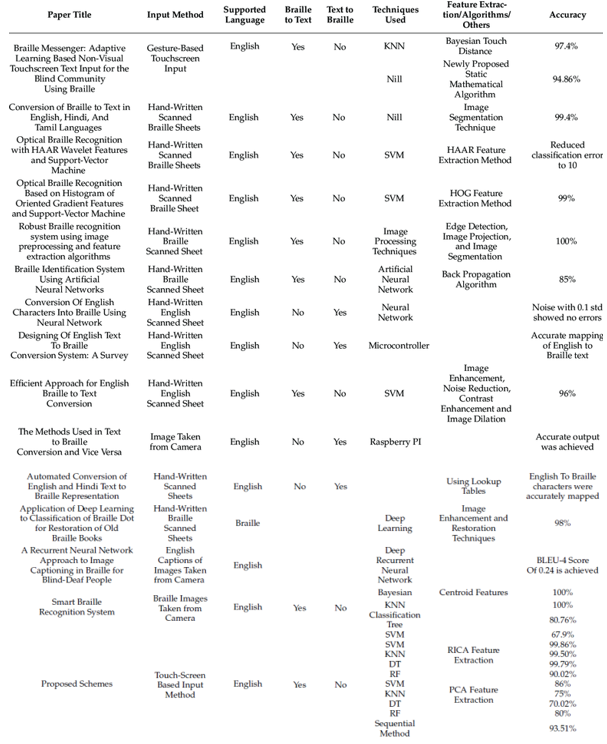
\includegraphics[width=\textwidth,height=22cm]{table 2.1.PNG} \\
        \hline
    \end{tabular}
    \caption{Comparative analysis of the feature Extraction/Detection techniques from previous studies }
    \label{tab: comparison}
\end{table}

\subsection{Text Correction Using Context}

One significant challenge in the translation of Braille to readable text is the issue of contextual accuracy. Misinterpretation of Braille dots can lead to incorrect characters, and without considering the context, words may be misinterpreted, particularly in languages with complex grammar. Additionally, Braille's specific formatting rules may not always translate seamlessly into text. Correcting these errors is crucial to ensure readability and accuracy. While standard spell checkers and grammar correction tools can address basic errors, they often fall short in understanding the context. This is where advanced methods, such as machine learning and contextual analysis, become essential. By leveraging neural networks and sequence-to-sequence models, it's possible to predict and correct errors based on the surrounding text. Contextual methods, such as n-grams and part-of-speech tagging, further enhance this process by providing a deeper understanding of sentence structure and word usage. However, even with sophisticated automated tools, human review remains invaluable for catching subtle errors. This highlights the need for a comprehensive approach to text correction that integrates automated tools with manual proofreading to ensure high-quality output. To delve deeper into the importance of context in spelling correction, we will discuss the findings from the paper titled "Spelling Correction Using Context" [9] which explores advanced techniques for enhancing text accuracy by focusing on the contextual relevance of words.

\paragraph{The system introduced by Elmi \& Evens}
 features an adaptive lexicon search and an intelligent filter to enhance processing speed. At its core, this approach leverages the interaction between a parser and a spelling corrector. The corrector proposes alternative spellings, which the parser then evaluates through syntactic and semantic checks within the dialogue, sentence, and phrase contexts.

Error detection is confined to isolated words. Once a misspelled word (S) is identified, the system follows a series of steps to find a suitable replacement. Initially, it selects a set of words from the lexicon for comparison. Then, it considers a configurable number of words similar to S as potential replacements. The final step involves using the sentence context to choose the best candidate, employing syntactic and semantic information along with phrase lookup to narrow down the options.

The system also allows users to set a limit on the number of errors. For a given limit (k), the program identifies all lexicon words that differ from the misspelled word by up to k mismatches, ensuring a comprehensive yet efficient correction process. This contextual approach significantly enhances the accuracy and reliability of the text correction, making it an invaluable tool for improving the readability of translated Braille text.\\

 

\subsection{Text to Speech}


 After successfully translating Braille text into readable text and ensuring accuracy through advanced correction techniques, the next crucial step in enabling accessibility for the visually impaired is converting this text into spoken language. This process, known as text-to-speech (TTS), plays a pivotal role in transforming written information into auditory output. Over the years, significant strides have been made in TTS technology, particularly through the pioneering work of researchers

\paragraph{Deep Voice, described in the research by Arık et al. [10]}
, represents an advanced neural network-based text-to-speech system designed for practical application. Unlike traditional methods that rely on complex feature engineering, Deep Voice utilizes deep neural networks across five core components. These include a model for phoneme boundary detection using connectionist temporal classification (CTC) loss, a grapheme-to-phoneme converter, models for predicting phoneme duration and fundamental frequency, and an efficient audio synthesis model inspired by WaveNet but with reduced complexity and faster training capabilities.

The use of neural networks in each component enhances the system's flexibility and simplifies its architecture compared to conventional text-to-speech systems. Importantly, the research demonstrates that the system can perform inference faster than real-time, showcasing optimized WaveNet inference kernels that achieve significant speed improvements on both CPU and GPU platforms. This innovation lays the groundwork for end-to-end neural speech synthesis, promising advancements in speech technology by leveraging deep learning techniques effectively.

The TTS system described in the Deep Voice paper comprises five integral components. First, the grapheme-to-phoneme model converts written text, represented in English characters, into phonemes using phonemic alphabet encoding like ARPABET. Subsequently, the segmentation model accurately identifies phoneme boundaries within voice datasets, pinpointing where each phoneme begins and ends in audio recordings. The phoneme duration model predicts the temporal length of each phoneme in an utterance, ensuring natural pacing and rhythm in synthesized speech. Meanwhile, the fundamental frequency model determines voicing and predicts fundamental frequency (F0) variations throughout phonemes, essential for generating lifelike intonation and pitch. Lastly, the audio synthesis model integrates outputs from the previous models to synthesize audio at a high sampling rate, aligning closely with the original text. During inference, text undergoes conversion into phonemes, followed by duration and F0 prediction, with these factors collectively conditioning the audio synthesis model to produce the final, coherent utterance.

\\
\paragraph{The Tacotron paper by Wang et al. [11]}
 introduces a groundbreaking approach towards achieving end-to-end speech synthesis directly from characters. Traditionally, such systems involve multiple stages including text analysis, acoustic modeling, and audio synthesis, each requiring specialized domain knowledge and often featuring rigid design choices. Tacotron, however, presents an innovative solution—a generative model that learns to synthesize speech from <text, audio> pairs starting from random initialization. The paper highlights several key techniques tailored for sequence-to-sequence learning, effectively addressing the complexities of this task. Notably, Tacotron achieves impressive results with a subjective mean opinion score of 3.82 on a 5-point scale for US English, surpassing the naturalness of existing parametric systems. Moreover, by generating speech at the frame level rather than sample-level autoregressive methods, Tacotron significantly enhances speed and efficiency in speech synthesis.

  As we conclude this comprehensive chapter, we have explored the intricate stages of optical Braille recognition from image preprocessing and filter application to precise Braille dot detection, symbol identification, and accurate symbol recognition. We have delved into the crucial aspect of text correction to ensure fidelity and accuracy in converting Braille symbols into readable text. Moreover, our journey has encompassed the transformative field of text-to-speech synthesis.

With these invaluable insights and methodologies at our disposal, our next ambition is to develop our own optical Braille recognition system. This system aims not only to convert images of Braille into correct textual representations but also to generate articulate speech, thereby enhancing accessibility for individuals with visual impairments. By leveraging advancements in image processing, machine learning, and speech synthesis techniques, we aspire to create a robust and inclusive solution that empowers users to access information independently and effectively. As we move forward into the next phase of development, we are dedicated to applying these lessons and exploring new possibilities to create solutions that are accessible to everyone.  